\documentclass[10pt]{beamer}

\usetheme[progressbar=frametitle]{metropolis}
\usepackage{appendixnumberbeamer}

\usepackage{booktabs}
\usepackage[scale=2]{ccicons}

\usepackage{pgfplots}
\usepgfplotslibrary{dateplot}

\usepackage{xspace}
\newcommand{\themename}{\textbf{\textsc{metropolis}}\xspace}

\usepackage{listings}
\usepackage{wrapfig}
\usepackage{subcaption}

\metroset{block=fill}


\title{Programmeringstävling Pepper}
\subtitle{Mattekollo}
\date{4e Augusti 2018}
%\date{}
\author{Fredrik Löfgren, Jinci Brettschneider, Jonatan Nilsson}
%\institute{Mattekollo}
% \titlegraphic{\hfill
\includegraphics[height=1.5cm]{logo.pdf}}

\begin{document}

\maketitle

\begin{frame}{Innehåll}
  \setbeamertemplate{section in toc}[sections numbered]
  \tableofcontents[hideallsubsections]
\end{frame}


\section{Regler}

\begin{frame}[fragile]{Vad får man använda?}

\begin{itemize}
\item Bara python 3.7 får användas (det som är installerat på skoldatorerna).
\item Inga andra bibliotek än de som finns på skoldatorerna (matplotlib, numpy, arcade är installerat förutom standard python) får användas. Vid tveksamheter ska vi kunna testa på en elevdator. Ni får självklart testa på såna i era grupper. 
\item Internet är tillåtet, men du måste kunna förklara din kod och svara på våra frågor för att få poäng. Du får inte sno \emph{hela} lösningar från nätet. Upptäcker vi fusk på någon uppgift kan ni inte få poäng på den uppgiften. 
\item Det är tillåtet att anteckna andras lösningar när de presenterar på tavlan, dels för att lära sig men också för att implementera deras algoritm smartare och tjäna mer poäng
\end{itemize}
\end{frame}

\begin{frame}[fragile]{Vilka jobbar?}

\begin{itemize}
\item Ni jobbar i grupper om 3 så långt det är möjligt. 
\item Vi har delat upp grupperna. 
\item Vi lärare kommer inte kunna hjälpa er med någon programmering, ni får fråga varandra i gruppen istället. Det enda vi kan svara på är frågor relaterat till problemformuleringarna. 
\end{itemize}
\end{frame}



\begin{frame}[fragile]{Hur fungerar tävlingen?}

\begin{itemize}
\item Ni får ett problem presenterat på projektorn. Det är relativt enkelt och vi bedömer att det i snitt tar 10 minuter att lösa på egen hand, men förhoppningsvis snabbare i grupp. 
\item Den som är klar med sin lösning först säger till oss ledare genom att skrika sitt gruppnamn. Då måste de släppa sina datorer och inte koda något mer. 
\item Gruppen som har en lösning får gå fram till tavlan och koppla in sin dator och starta sitt program. Sen kommer en ledare att testa det med testfall som vi bestämmer. Programmet ska gå att förstå och använda för oss (behöver inte vara snyggt).
\item Om programmet klarar testfallen så ska ni presentera er kod för de andra deltagarna. Om det inte fungerar / klarar testfallen får ni gå och sätta er igen utan att presentera er kod. 
\end{itemize} 
\end{frame}




\begin{frame}[fragile]{Poängräkning?}

\begin{itemize}
\item Om ni inte kan förklara er kod tillräckligt bra (bedöms av lärarna) så får ni 0 poäng för det försöket. Ingen annan får heller poäng. 
\item Om ni har rätt på testfallen och kan förklara er kod får ni 100 poäng. 
\item Om programmet tar mer än ca 30s att köra, så får ni 0 poäng. Våra exempellösningar går oftast på $\le1$s.
\item Om ni har fel på testfallen så får alla andra tävlande lag 100 poäng. Detta för att ni inte ska chansa och gå fram för tidigt och slösa vår värdefulla tid. 
\end{itemize}
\end{frame}



\begin{frame}[fragile]{Poängräkning - special!}

\begin{itemize}
\item Vissa lag kanske bara hade någon rad kvar innan ett annat lag blev klara och fick presentera. Istället för att slänga bort allt ert fantastiska arbete så ger vi er chansen att visa upp det och ändå få poäng, under förutsättning att er kod är kortare (färre bytes) än de som tidigare presenterat. 
\item Vi är medvetna om att kort kod inte alltid betyder bra kod, men det är enklare att mäta än tidsåtgången då ni kör på olika datorer. Dessutom finns det många tävlingar där man ska skriva så kort kod som möjligt.
\end{itemize}

\end{frame}




\begin{frame}[fragile]{Poängräkning - special!}

\begin{itemize}
\item För en korrekt visad lösning som ni kan förklara får ni hälften av poängen som delades ut innan på den här uppgiften.  
\item För en lösning som inte klarar testfallen så får alla andra lagen hälften av det som delades ut innan på den här uppgiften. 
\item Ni kan fortsätta att förkorta lösningar och få hälften av poängen igen. Men ni kan aldrig presentera igen på en uppgift som ni redan klarat testfallen på (oavsett om ni kunde förklara er kod och fick full poäng, eller inte klarade och fick 0 poäng). Har ni däremot haft fel på testfallen, och gett alla andra lag poäng, kan ni fortsätta testa på den uppgiften.
\end{itemize}
\end{frame}




\begin{frame}[fragile]{Hur fortsätter det?}

\begin{itemize}
\item Varje gång någon har klarat testfallen och presenterat korrekt för ett problem så kommer vi släppa ett nytt problem på projektorn. Vi presenterar inte ett nytt problem när någon lyckas visa en ny kortare lösning på ett redan avklarat problem.
\item Ni får fota eller skriva av problemformuleringen för vi kan inte gå fram och tillbaka mellan problemen hela tiden. 
\item Ni får alltså fler och fler problem att lösa, och ni kan alltid fortsätta att försöka på problem som ni tidigare inte klarat för att lyckas få halva poäng (vilket fortfarande är rätt mycket!).
\end{itemize}
\end{frame}





\begin{frame}[fragile]{Exempel!}

\begin{itemize}
\item Vi har lag A, B, C.  De får ett problem I. 
\item Lag C säger att de klarat uppgiften och går fram och presenterar, de lyckas både med testfall och att förklara sin kod och får 100 poäng. 
\item Ett problem II presenteras och lag B delar upp sig så att två personer satsar på det nya medan en fortsätter med problem I. Lag A förstår inte det nya problemet så alla sitter kvar med problem I. 
\item Lag A skriker att de är klara och får presentera sitt problem. De lyckas och får 50 poäng. Inget nytt problem presenteras då problem I redan är löst.
\item Lag B är klara med problem II, de lyckas med alla testfall och presentationen och får därmed sina första 100 poäng! 
\item Problem III presenteras.
\item Lag B säger att de är klara med problem III, men har tyvärr fel och ger alla andra lag 100 poäng. Inget nytt problem presenteras då. 
\item Lag B säger igen att de är klara, nu på problem I som en ensam stackare jobbat på. De lyckas med testfallet och får 25 poäng! 
\end{itemize}
\end{frame}





\begin{frame}[fragile]{Frågor?!}

Något som är oklart innan vi sätter igång? 

\end{frame}




\section{Då börjar vi!}


\begin{frame}{Valentinas choklad}

Valentina tycker om choklad. Hon har därför alltid en öppnad chokladkartong i skafferiet. När den tar slut köper hon i hemlighet en ny och låtsas som ingenting. Valentinas bror Danil, som är misstänksam av naturen, förundras över att den där kartongen aldrig tar slut. Därför börjar han vid varje besök att räkna antalet chokladbitar som är kvar. Skriv ett program som, givet hans observationer, beräknar det minsta antalet nya kartonger Valentina måste ha köpt under perioden. 

\begin{exampleblock}{Indata}
Tar in $N$ heltal (lika många heltal som observationer), där heltalen motsvarar antalet chokladbitar i asken (mellan 1 och 100) vid varje observation, i den ordning de görs.
\end{exampleblock}

\begin{exampleblock}{Utdata}
Programmet ska skriva ut ett heltal: det minsta antal nya kartonger Valentina bevisligen måste ha köpt under perioden.
\end{exampleblock}

%\textbf{Körningsexempel:}
%\begin{lstlisting}
%Observationer ? 17 15 16 16 18 17 14 12 13 9
%Valentina måste åtminstone ha köpt 3 chokladaskar.
%\end{lstlisting}
\end{frame}



\begin{frame}{Blockpyramid}

\begin{figure}[!ht]
\centering
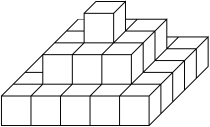
\includegraphics[width=0.3\textwidth]{pyramid.png}
%\caption{Denna pyramid med höjden 3 innehåller 35 stenblock. Cheopspyramiden i Egypten har höjden 210.}
\label{fig:begransningsarea}
\end{figure}

Du ska skriva ett program som beräknar hur hög pyramid man kan bygga om man har tillgång till ett visst antal stenblock.

Vi antar att pyramiden är kompakt, d.v.s. det finns inga hålrum inuti. Vidare byggs den enligt principen i figuren ovan. Varje lager är alltså kvadratiskt med en sidlängd som är två block mindre än det underliggande lagrets. Det översta lagret består alltid av ett ensamt block.

Programmet ska fråga efter antalet tillgängliga block (högst hundra miljoner) och skriva ut höjden (i block räknat) för den största pyramid som kan byggas. Det gör ingenting om det blir block över, men det får inte saknas ett enda block.

\end{frame}





\begin{frame}{Leonids valkampanj}

Leonid kandiderar till ordförandeposten i matematiksällskapet och vill inte riskera att förlora omröstningen. Han har lyckats få reda på vilken kandidat varje medlem tänker rösta på och tänker helt enkelt muta ett antal medlemmar så att de röstar på honom istället. Skriv ett program som beräknar hur många röster som måste köpas (d.v.s. medlemmar som behöver mutas) för att Leonid ska vinna omröstningen. För att vinna krävs att man får fler röster än var och en av de andra kandidaterna.

\begin{exampleblock}{Indata}
Först ska man mata in antal kandidater ($1 \le n \le 20$). Sedan ska man mata in $n$ heltal (mellan 0 och 1000): antalet röster varje kandidat skulle få utan mutor. Det första talet anger Leonids röster.
\end{exampleblock}

\begin{exampleblock}{Utdata}
Programmet ska skriva ut ett heltal: det minsta antalet röster som behöver köpas för att Leonid ska få fler röster än var och en av de övriga kandidaterna.
\end{exampleblock}

\end{frame}




\begin{frame}{Röd, grön, blå}
\begin{itemize}
\item Röda block har längd 2.
\item Gröna block har längd 3.
\item Blåa block har längd 4.
\end{itemize}

På en sträcka av längd 5 kan man placera in röda,gröna och blåa block på exakt 15 olika sätt:

\begin{figure}[!ht]
\centering
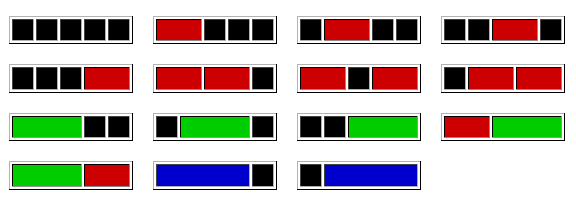
\includegraphics[width=0.3\textwidth]{blarodgron}
%\caption{15 olika sätt att lägga ut på en sträcka av längd 5.}
\label{fig:bocker}
\end{figure}


Hur många sätt kan man placera ut röda, gröna och blåa block på en sträcka av längd N?
\end{frame}






\begin{frame}{Klockan}

\begin{figure}[!ht]
\centering
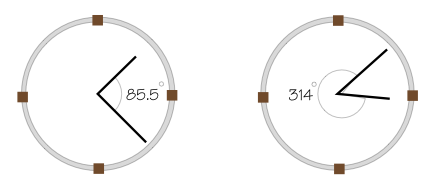
\includegraphics[width=0.4\textwidth]{klocka}
%\caption{}
\label{fig:klocka}
\end{figure}

Man kan ange ett klockslag med vinkeln mellan tim- och minutvisaren, eftersom man ur denna information entydigt kan bestämma klockslaget.

Vi förutsätter att vår klocka saknar sekundvisare och endast visar ett helt antal minuter (det vill säga: båda visarna hoppar framåt bara på hel minut). Vinkeln avläses genom att utgå från timvisaren och sedan mäta hur många grader medurs minutvisaren ligger. Som en följd av att endast hela minuter visas, är vinkeln alltid en multipel av 0.5.

Programmet ska fråga efter en vinkel och sedan skriva ut tiden i vanligt digitalformat, alltså h:mm eller hh:mm, alla tider ska ligga mellan 0:00 och 11:59 (inklusive).

\end{frame}



\begin{frame}{Begränsningsarea}

\begin{figure}[!ht]
    \centering
    \begin{subfigure}[b]{0.3\textwidth}
        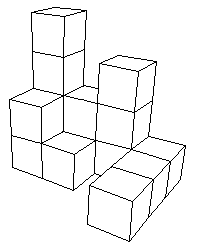
\includegraphics[height=\textwidth]{begransningsarea.png}
        \label{fig:begransningsarea}
    \end{subfigure}
    ~ %add desired spacing between images, e. g. ~, \quad, \qquad, \hfill etc. 
      %(or a blank line to force the subfigure onto a new line)
    \begin{subfigure}[b]{0.3\textwidth}
        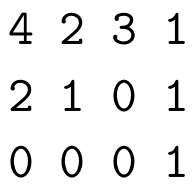
\includegraphics[height=\textwidth]{begransningsarea_input}
        \label{fig:begransningsarea_input}
    \end{subfigure}
\end{figure}



Betrakta den tredimensionella figuren ovan. Den är ihopsatt av ett antal $1\times1\times1$ kuber i ett 3d-rutnät. Vi begränsar oss till figurer som har staplar fästa i ''marken'', så ingen kub har luft under sig. 

Figurens volym är förstås enkel att beräkna, men här är vi intresserade av dess begränsningsarea, d.v.s. antalet $1\times1$ kvadrater som är synliga utifrån (inklusive underifrån). Skriv ett program som beräknar detta, givet beskrivningen av en figur.
Figurens basarea kan maximalt vara $50\times50$, och staplarnas höjd är maximalt 50. 

\end{frame}










\begin{frame}{Egyptisk matematik}

I egyptisk matematik hade de så kallade heltalsreciprokerna

${\displaystyle {\frac {1}{1}},{\frac {1}{2}},{\frac {1}{3}},{\frac {1}{4}},...}$

särskild betydelse. Övriga bråk skrevs som summor av dessa tal, t.ex.

${\displaystyle {\frac {21}{20}}={\frac {1}{2}}+{\frac {1}{4}}+{\frac {1}{5}}+{\frac {1}{10}}}$

Skriv ett program som tar emot ett bråk (förkortat så långt som möjligt) och avgör om det kan skrivas som en sådan summa, under villkoren att bara de tio första heltalsreciprokerna (alltså t.o.m. 1/10) får användas, och att varje tal endast får användas en gång. Om det går ska programmet skriva ut de ingående termerna i summan, annars ska det skriva ut Omöjligt. Om det finns flera lösningar ska programmet skriva ut vilken som helst av dem.

\end{frame}








\begin{frame}{Sfnix-sex}

En sfinx är en varelse med ett lejons kropp och en människas huvud.

Vi antar att när två kombinationsvarelser parar sig så ärver avkomman framkroppen från den ena föräldern och bakkroppen från den andra. En grodmus som parar sig med en fiskhöna kan alltså ge upphov till antingen en grodhöna eller en fiskmus.

Skriv ett program som, givet en grupp kombinationsvarelser (somliga hannar och andra honor) beräknar antalet olika arter som kan existera i nästa generation om alla par av hanne-hona antas få ungar.

Programmet ska fråga efter antalet hannar och vilken art varje hanne tillhör, samt likadant för honorna. Arten anges som en sträng med två bokstäver (valda bland A-Z), där första bokstaven beskriver framkroppen och andra bokstaven bakkroppen (t.ex. ML för människolejon). Programmet ska skriva ut det totala antalet olika arter som kan finnas när parning har skett. Observera att ordningen på bokstäverna spelar roll – MF och FM är olika arter.

\end{frame}






\begin{frame}{Förvirrade soldater}

%\begin{figure}[!ht]
%\centering
%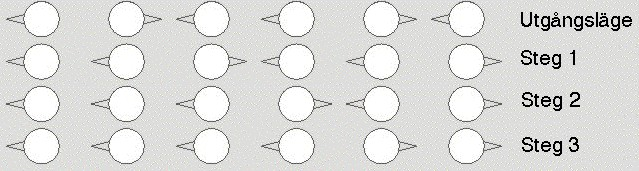
\includegraphics[width=0.4\textwidth]{soldater.jpg}
%\caption{Uppställning av soldater}
%\label{fig:soldater}
%\end{figure}

Ett antal soldater står på ett led alla vända mot furiren, när han ger ordern ''höger om''. Eftersom många av soldaterna har svårt att skilja på höger och vänster blir det mest slumpen som avgör åt vilket håll de vänder sig. De soldater som på så sätt hamnar ''öga mot öga'' med en granne förstår båda två att de vänt sig åt fel håll och gör därför helt om (180 grader), för att kanske hamna öga mot öga med den andra grannen. Denna procedur fortsätter tills inga soldater längre är vända mot varandra.

\begin{exampleblock}{Indata}
En rad där varje tecken är antingen V eller H. Dessa anger åt vilket håll soldatens näsa pekar i utgångsläget. Maximalt 100 tecken. 
\end{exampleblock}

\begin{exampleblock}{Utdata}
Programmet ska skriva ut hur många steg som behövs från utgångsläget tills lugnet infinner sig.
\end{exampleblock}

\end{frame}







\begin{frame}{Send more money}

Ersätt varje bokstav med en unik siffra mellan 0 och 9 så att uträkningen nedan stämmer. Notera att talen inte kan börja med 0, för i så fall skulle man kunna strunta i att skriva ut första bokstaven. 

\begin{figure}[!ht]
\centering
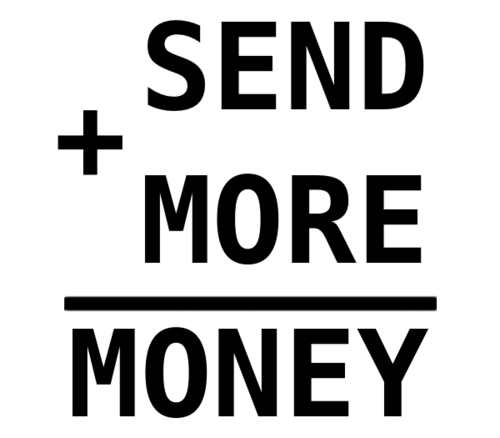
\includegraphics[width=0.3\textwidth]{sendmoremoney}
%\caption{}
\label{sendmoremoney}
\end{figure}

\end{frame}







\begin{frame}{Busig dotter}

En bonde har fem höbalar. Han bad sin dotter som deltagit på mattekollo att väga upp balarna åt honom, men istället för att väga dem en och en, valde hon att väga dem i parvisa kombinationer: bal 1 och 2, bal 1 och 3, bal 1 och 4, bal 1 och 5, bal 2 och 3, bal 2 och 4, osv. 

Vikterna för dessa parvisa vägningar skrev hon upp på 10 papperslappar. Men sen glömde hon bort vilken lapp som hörde till vilket par så hon tänkte ''Äsch, det spelar ju ingen roll, jag lägger dem i storleksordning.''

Nu står bonden här och har ingen aning om vilken höbal som väger vad. Det enda han har är papperslapparna. Ingen av lapparna har ett tal större än 100 och alla lappar har olika tal. Kan du  hjälpa honom att reda ut det här? Hur mycket väger varje höbal? Finns det fler en än lösning? 

\end{frame}






\begin{frame}{Lagomvinklade trianglar}

En lagomvinklad triangel är vad vi i denna uppgift kallar en triangel där minst en av vinklarna är exakt 60 grader. De lagomvinklade har en snygg formel för sina sidlängder:

${\displaystyle c^{2}=a^{2}+b^{2}-ab}$

Skriv ett program som frågar efter ett tal N (mellan 1 och 100) och sedan skriver ut hur många unika lagomvinklade trianglar det finns vars sidor är heltal i intervallet 1 till N.

\begin{figure}[!ht]
\centering
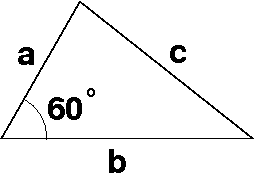
\includegraphics[width=0.3\textwidth]{triangel}
\caption{Ett exempel på en lagomvinklad triangel med sidlängderna $a = 5, b = 8$ och $c = 7$.}
\label{triangel}
\end{figure}
\end{frame}









\begin{frame}{Uppställning}

En patrull på mattekollo med 10 ungdomar bestämmer sig för att utmana sin ledare. Utan att hen ser dem så ställer de sig på en rad och räknar hur många av de ungdomar som står till vänster om honom/henne som är längre än han/hon själv, och sedan likadant med dem som står till höger. Var och en skriver ner dessa antal på en lapp som de ger till ledaren. Deras enkla uppmaning till henom är att tala om i vilken ordning de stod.

Tyvärr klarade ledaren inte nöten utan måste i hemlighet smyga iväg och be dig att skriva ett datorprogram som löser uppgiften. Du kan förutsätta att alla barn är olika långa och att de inte har gjort något misstag när de skrev lapparna. Intressant nog finns det aldrig mer än en lösning. 

\end{frame}








\begin{frame}{Snöskottning}

Scotts hus måste skottas ofta, men han tycker själv att skotta varje dag är för ofta. Du ska hjälpa Scott att sätta upp ett skott-schema för de kommande N dagarna. Till din hjälp har du en detaljerad väderleksprognos, så du vet exakt hur många cm det snöar eller smälter varje dag (innan kvällen). När det ligger minst H cm snö en kväll så är det dags att skotta, och när man skottar så försvinner all snö. Från början är det ingen snö alls.

\begin{exampleblock}{Indata}
Första raden innehåller antalet dagar $1 \le N \le 100$ och andra raden snötröskeln $1 \le H \le 1000$. Därefter följer N heltal mellan $-100$ och $100$ (inklusive). Dessa tal beskriver hur många cm snö det kommer under var och en av de kommande N dagarna. Ett negativt värde betyder att denna mängd smälter istället (men snötäcket kan naturligtvis aldrig bli mindre än 0).
\end{exampleblock}

\begin{exampleblock}{Utdata}
Utdatat ska bestå av ett heltal, antalet kvällar Scott måste skotta.
\end{exampleblock}

\end{frame}





\begin{frame}{Kölappar}

Du råkar gå till banken i rusningstid. Ett vanligt kölapps-system används, men $n$ kunder har lägre könummer än du. Dock är $m$ kassor öppna. Skriv ett program som, givet hur lång tid varje kunds ärende tar, beräknar hur lång tid det tar innan det är din tur.

Varje kund har ett bankärende som tar ett helt antal minuter. Så fort det finns en ledig kassa kallas nästa person i kön fram. Kundbytet tar inget tid i anspråk. För enkelhets skull förutsätter vi att i det ögonblicket du tar din kölapp, låt oss kalla det tiden 0, så är alla kassorna lediga och m kunder kallas alltså fram omedelbart.

\begin{exampleblock}{Indata}
Antalet personer före dig i kön ($1 \le n \le 100$) och antalet öppna kassor ($1 \le m \le 10$). Därefter följer en rad med $n$ heltal i intervallet 1..20, antalet minuter för varje kunds ärende.
\end{exampleblock}

\begin{exampleblock}{Utdata}
Efter hur många minuter du får påbörja ditt ärende.
\end{exampleblock}

\end{frame}









\begin{frame}{Tågväxeln}

Tågstationen hade två linjer, och tågen gick periodiskt med $m$ respektive $n$ minuters mellanrum, med första avgång $m$ respektive $n$ minuter efter midnatt. Alla tåg åkte alltså ut från stationen åt samma håll men delades sedan upp på två olika spår med hjälp av en växel. 

Hur många gånger måste växeln ändras under ett helt dygn? Tågen avgår alltså bara under minuterna 00:00 till 23:59.

\begin{enumerate}
\item Om ett tåg avgår, och växeln är fel inställd, måste den ändras till rätt spår.
\item Om båda tågen avgår samma minut, så avgår först det tåg som växeln är inställd för, och sedan ska den ändras till det andra tågets spår.
\end{enumerate}

I början var växeln inställd på spåret för det tåg som avgår först.

Skriv ett program som beräknar hur många gånger som växeln måste ändras under ett helt dygn.


\end{frame}









\begin{frame}{Robotskattjakt}

En robot ska följa pilar på en rektangulär skattkarta. Roboten börjar alltid i den ruta som befinner sig längst upp till vänster på skattkartan, och följer därefter pilarna. I labyrinten finns det två olika mål: ett batteri, samt en läskig elstöt. Det kan också hända att skattkartan leder runt roboten i en oändlig cykel av rutor så den aldrig når ett mål.


\begin{wrapfigure}{r}{0.2\textwidth}
    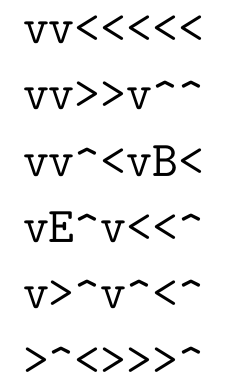
\includegraphics[width=0.2\textwidth]{karta}
  %\caption{A gull}
\end{wrapfigure}

Kan du hjälpa roboten att avgöra vilket mål den når, eller om den kommer gå runt i all oändlighet.


Följande tecken förekommer i skattkartan:
\begin{itemize}
\item ''<'' – ruta med vänsterpil,
\item ''>'' – ruta med högerpil,
\item ''v'' – ruta med nedåtpil,
\item ''\^{}'' – ruta med uppåtpil,
\item ''B'' – rutan batteriet befinner sig på,
\item ''E'' – rutan elstöten befinner sig på.
\end{itemize}

\end{frame}








\begin{frame}{Tvetydiga datum}

Datum skrivs på olika sätt i olika länder. Till exempel skulle datumet 03/05/01 i Sverige betyda 1 maj 2003, medan det i USA skulle vara 5 mars 2001 och i en del andra länder 3 maj 2001 (vi kan utgå ifrån att årtalet alltid är under 2000-talet, dvs mellan 2000 och 2099).

Detta kan bland annat orsaka bekymmer när man tittar på bäst-före datumet på en gammal konservburk. Om man inte har en aning om vilket format ett datum har, kan man behöva pröva alla möjliga betydelser och, för att vara på den säkra sidan, välja det tidigaste giltiga datumet.

Skriv ett program som läser in de tre delarna av ett datum (varje del kan max vara 99, men självklart inte samtidigt) och skriver ut det tidigaste giltiga datumet som indata kan tänkas representera.

\end{frame}





\begin{frame}{Travar med böcker}


\begin{figure}[!ht]
\centering
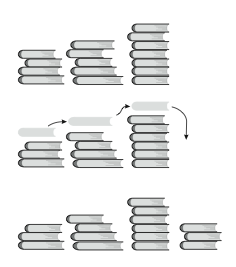
\includegraphics[width=0.25\textwidth]{Travar}
%\caption{Första dagen plockas en bok från var och en av de tre travarna. Dessa tre böcker bildar en ny trave till höger om de andra.}
\label{fig:bocker}
\end{figure}

På ett bord ligger att antal travar med böcker. Varje dag tas en bok från varje trave. Dessa böcker bildar tillsammans en ny trave till höger om de andra. Om en trave blir tom skjuts travarna samman från höger. Eftersom det finns ett ändligt antal böcker, kommer förr eller senare samma upplägg att återkomma. Skriv ett program som frågar efter första uppläggets utseende och tar reda på hur lång tid det tar innan ett upplägg som tidigare funnits, återkommer.

I testfallen är antalet böcker $\le50$, antalet travar som mest $\le15$ och antalet dagar $\le100$.
\end{frame}


\begin{frame}[fragile]{XKCD 710}

\begin{wrapfigure}{r}{0.33\textwidth}
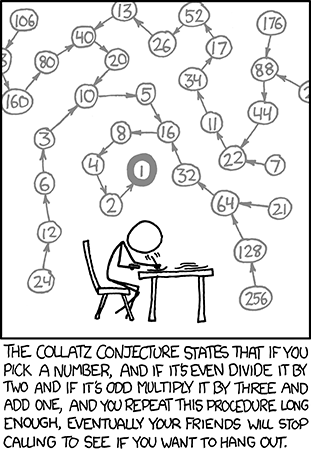
\includegraphics[width=0.33\textwidth]{collatz_conjecture}
%\caption{A gull}
\end{wrapfigure}

Tänk dig att du skriver upp alla positiva heltal på ett oändligt stort papper. Från varje tal $n>1$ ritar du nu en pil till talet

\begin{itemize}
\item $n/2$ om $n$ är jämnt.
\item $3n+1$ om $n$ är udda.
\end{itemize}

De talföljder man får genom att följa pilarna kallas ibland för hageltal eftersom de likt hagelkorn driver upp och ner längs tallinjen innan de slutligen faller ner till marken (talet 1). 

Skriv ett program som, givet två olika heltal beräknar hur långt ifrån varandra (antal pilar, oavsett riktning) de är i grafen. 
\end{frame}




\section{Resultat?}


{\setbeamercolor{palette primary}{fg=black, bg=yellow}
\begin{frame}[standout]
  Tack för att ni deltog!
\end{frame}
}

\end{document}
